\documentclass[12pt, oneside, openany]{book}

\usepackage{mathptmx} % Contiene una fuente similar a Times New Roman

\usepackage[spanish, es-tabla]{babel} % Permite escritura en castellano
\usepackage[utf8]{inputenc} % Permite utilizar caracteres UTF8

\usepackage{graphicx} % Para la inclusión de gráficos e imágenes
\graphicspath{ {images/} } % Ruta para buscar las imágenes
\usepackage[a4paper,top=30mm,left=30mm,right=25mm,bottom=25mm,headheight=20mm]{geometry} % Configuración de los margenes de la página

% Paquetes para que funcione el formato.
\usepackage{titlesec}
\usepackage{setspace}
\usepackage{ragged2e}
\usepackage{fancyhdr}
\usepackage{lastpage}
\usepackage{stackengine}
\usepackage{array}
\usepackage[hidelinks]{hyperref}
\usepackage{enumitem}
\usepackage{float}
\usepackage{hypcap}
\usepackage{caption}
\usepackage{fancyvrb}
\usepackage{amsfonts}
\usepackage{tabularx}
\usepackage{multirow}
\usepackage{hyperref} % Paquete para que las referencias funcionen, y permite introducir links
\usepackage[table]{xcolor} % Paquete para trabajar con colores (fondo de celdas, color del texto...)
\usepackage{tcolorbox}
% Se define un color gris desde su código RGB
\definecolor{gris}{RGB}{220,220,220}

\setcounter{secnumdepth}{3} % Para permitir numerar las sub-subsecciones

% Modifica el nombre de los índices al castellano
\addto\captionsspanish{
  \renewcommand{\contentsname}{Índice de contenido}
  \renewcommand{\listfigurename}{Índice de figuras}
  \renewcommand{\listtablename}{Índice de tablas}
}

% Formateo de los nombres de los apartados:
\titleformat{\chapter}[block]
  {\normalfont\Huge\bfseries\singlespacing}{\thechapter.}{1em}{\Huge}
\titlespacing*{\chapter}{0pt}{-62pt}{0pt}

\titleformat{\section}[block]
  {\normalfont\Large\bfseries}{\thesection.}{4pt}{\Large}
\titlespacing*{\section}{0pt}{\baselineskip}{0pt}

\titleformat{\subsection}[block]
  {\normalfont\large\bfseries}{\thesubsection.}{4pt}{\normalsize\large}
\titlespacing*{\subsection}{0pt}{0pt}{0pt}

\titleformat{\subsubsection}[block]
  {\normalfont\normalsize\bfseries}{\thesubsubsection.}{4pt}{\normalsize}
\titlespacing*{\subsubsection}{0pt}{0pt}{0pt}

\def\tablename{Tabla}

%% Variables para portada y cabeceras
%% Cambiar los valores para cada documento!!!
\def\title{Ejercicio Teórico 2}
\def\subject{Pruebas y Despliegue de Software}
\def\author{Juan Francisco Mier Montoto}
\def\target{www.mier.info}
\def\authorid{UO283319}
\def\date{mayo 2024}
\def\org{Escuela Politécnica de Ingeniería de Gijón}
\def\area{Grado en Ingeniería Informática en Tecnologías de la Información}

\def\ORG{\expandafter\MakeUppercase\expandafter{\org}}
\def\AREA{\expandafter\MakeUppercase\expandafter{\area}}
\def\SUBJECT{\expandafter\MakeUppercase\expandafter{\subject}}

\captionsetup{justification=centering}
\setlength{\headheight}{65pt}

\fancyhf{}
\fancyhead[L]{
\includegraphics[height=16mm]{style/square.png}
  \hspace{1em} \Longstack[l] {
    \textbf{\SUBJECT} \newline
    \textbf{\title}}
  \newline \leftmark{}
}
\fancyhead[R]{\bfseries{Hoja \hyperlink{toc}{\thepage}~de~\pageref{LastPage}}}
\fancyfoot[C]{\href{\target}{\author}}
\renewcommand{\headrulewidth}{0pt} % default is 0pt
\renewcommand{\footrulewidth}{0.4pt} % default is 0

\fancypagestyle{plain}{%
  \fancyhf{}
  \fancyhead[L]{
\includegraphics[height=16mm]{style/square.png}
    \hspace{1em} \Longstack[l]{
      \textbf{\SUBJECT} \newline
      \textbf{\title}}}
  \fancyhead[R]{\bfseries{Hoja \hyperlink{toc}{\thepage}~de~\pageref{LastPage}}}
  \fancyfoot[C]{\href{\target}{\author}}
  \renewcommand{\headrulewidth}{0pt} % default is 0pt
  \renewcommand{\footrulewidth}{0.4pt} % default is 0pt
}

\pagestyle{fancy}

\restylefloat{table}



\begin{document}

\rmfamily % Fuente tipo Romana

% Portada de la memoria
\begin{titlepage}
    \centering
    \bfseries {
        \null{}
        \vspace{0cm}
        \begin{table}[h]
            \centering
            \begin{tabular}{m{10cm} m{1cm} m{3cm}}
                \vspace{0.2cm}
                
\includegraphics[width=86mm]{style/full.png} &  & \vspace{1.52mm} 
\includegraphics[width=23mm]{style/square.png} \\
            \end{tabular}
        \end{table}

        \vspace{3\baselineskip}

        \Large{\ORG{} \\ \vspace{3\baselineskip}}
        \large {
            \AREA{} \\ \vspace{3\baselineskip}
            \subject{} \\ \vspace{2\baselineskip}

            % TRABAJO FIN DE GRADO/MÁSTER Nº XXXXXXXXX \vspace{\baselineskip} \\
            \title{} \\ \vspace{3\baselineskip}

            \author{} \\
            \authorid{} \\
            % TUTOR/ES: \\
            % D. APELLIDO1 APELLIDO2, Nombre \\
            % D. APELLIDO1 APELLIDO2, Nombre \\  \vspace{\baselineskip}

            \vspace{2\baselineskip}
            FECHA:\@ \date{}
        }
    }
\end{titlepage}


% Índice de contenido
\addcontentsline{toc}{chapter}{Índice de contenido} % Añade la referencia al índice de contenido
\hypertarget{toc}{}
\tableofcontents
\newpage{}

% Índice de figuras
\addcontentsline{toc}{chapter}{Índice de figuras}  % Añade la referencia al índice de contenido
\hypertarget{lof}{}
\listoffigures

\justify{} % Texto justificado
\setlength{\parskip}{\baselineskip} % Separación entre párrafos de 1 linea
\onehalfspacing{}

%% El contenido de la memoria, dividido en capítulos:
\chapter{Introducción}
En este documento se detalla el diseño de pruebas para un sistema de cálculo de retenciones de IRPF.~El sistema
debe ser capaz de calcular las retenciones de IRPF a aplicar a un trabajador en función de su base imponible,
retenciones, número de empleadores y préstamos hipotecarios.

Este sistema está descrito en el enunciado del primer ejercicio~\cite{enunciado1} y expandido en el enunciado
del segundo ejercicio~\cite{enunciado2}, sobre el que se basa este documento.

\chapter{Clases de equivalencia}
Según la descripción del sistema que otorga el enunciado, se identifican los siguientes conjuntos de entradas
que definen las clases de equivalencia. Para definir las clases de equivalencia se utiliza una sintaxis
matemática, donde se define el conjunto de valores que pertenecen a las mismas.

A continuación se definen las clases de equivalencia para las entradas y salidas del sistema:

\section{Entradas}
\subsection{Base imponible ($BI$)}
La base imponible se toma como la suma de ingresos de todos los empleadores
(en caso de tener más de uno) y se define por tramos según el enunciado.
A esta suma ``total'' se le denomina $BI$.

Puesto que puede haber un número (teóricamente) \textit{infinito} de pagadores,
se acumulan todos los ingresos de los empleadores \textit{secundarios} (es decir, que no
son los principales) en una variable $BI_{o}$, mientras que el principal se define como $BI_{p}$.

\begin{enumerate}
	\item $BI \in [0, 9000)$€
	\item $BI \in [9000, 12450)$€
	\item $BI \in [12450, 20200)$€
	\item $BI \in [20200, 35200)$€
	\item $BI \in [35200, 60000)$€
	\item $BI \in [60000, 300000)$€
	\item $BI \in [300000, \infty)$€
	\item $BI \notin \mathbb{R}, BI < 0$€ (\textcolor{red}{Inválido})
\end{enumerate}


\subsection{Retenciones ($R$)}
Donde $I$ es el cálculo de impuestos a pagar. Al igual que con la base imponible, se definen
dos variables para las retenciones: $R_{o}$ para la suma de las retenciones que realizan los
empleadores secundarios y $R_{p}$ para el empleador principal.

\begin{enumerate}
	\item $R \in [0, I)$€
	\item $R \in (I, \infty)$€
	\item $R = I$€
	\item $R \notin \mathbb{R}, R < 0$€ (\textcolor{red}{Inválido})
\end{enumerate}

\subsection{Préstamos hipotecarios ($P_{H}$)}
En este caso, se define $P_{H}$ como la cantidad de dinero que se ha pagado
en concepto de préstamos hipotecarios en viviendas habituales anteriores a 2013.

$60266$€ es el valor por encima del cual se dejaría de aplicar la deducción por vivienda habitual,
que resulta del siguiente cálculo: $$\frac{9040}{0.15} = 60266.66666\dots$$

\begin{enumerate}
	\item $P_{H} = 0$€
	\item $P_{H} \in (0, 60266]$€
	\item $P_{H} \in (60266, \infty)$€
	\item $P_{H} \notin \mathbb{R}, P_{H} < 0$€ (\textcolor{red}{Inválido})
\end{enumerate}

El valor máximo de la deducción es 9040€, lo que no significa que por encima de dicho valor no se aplique
la deducción, sino que el valor de la deducción no aumenta por encima de dicho valor.

\newpage{}
\section{Salidas}
\subsection{Obligatoriedad de la declaración}
\begin{itemize}
	\item Obligatorio
	\item No obligatorio
\end{itemize}

\subsection{Deducciones}
Resume las deducciones que se aplican a la declaración, que en el caso de este enunciado
es solo la deducción por préstamos hipotecarios.

Puesto que solo se tiene en cuenta una deducción, el cálculo debe de caer en el rango
de valores $[0, 9040]$\texteuro.

\subsection{Liquidación final}
El cálculo de la declaración se realiza en base a las retenciones y la base imponible por \textit{tramos}
tal y como define el enunciado, por lo que la salida del cálculo final dependerá de los valores
de las entradas.

Esta salida tiene especial conexión con la entrada $R$, ya que el cálculo de la declaración
depende directamente de la cantidad de retenciones que se han realizado. Al cálculo final de esta salida
deberían aplicarse las deducciones correspondientes (en este enunciado solo se considera $P_{H}$), es
decir, la clase de salida anterior.

\chapter{Técnicas de pruebas}
\section{Análisis de valores límite}
Para el análisis de valores límite, se han seleccionado los valores límite de las clases de equivalencia
de entrada definidas en el capítulo anterior, poniendo especial atención al cumplimiento de las aperturas
de los intervalos.

\subsection{Base imponible ($BI$)}
Debido a la naturaleza de esta variable, se han seleccionado los valores límite de los intervalos definidos
anteriormente.
\begin{itemize}
	\item $BI = 0$€
	\item $BI = 8999$€
	\item $BI = 9000$€
	\item $BI = 12449$€
	\item $BI = 12450$€
	\item $BI = 20199$€
	\item $BI = 20200$€
	\item $BI = 35199$€
	\item $BI = 35200$€
	\item $BI = 59999$€
	\item $BI = 60000$€
	\item $BI = 299999$€
	\item $BI = 300000$€
\end{itemize}

Como especificado en el análisis de clases de equivalencia, el valor $BI$ es la suma de todas
las bases imponibles de los empleadores, que se dividen en dos categorías: el empleador principal
$BI_{p}$ y los empleadores secundarios $BI_{s}$.

\newpage{}
\subsection{Retenciones ($R$)}
Esta variable es especialmente interesante para el AVL, ya que el cálculo de las retenciones depende
directamente de la base imponible, por lo que debería haber una relación directa entre los valores límite
de ambas variables.

\begin{itemize}
	\item $R = 0$€
	\item $R = I - 1$€
	\item $R = I$€
	\item $R = I + 1$€
\end{itemize}

Al igual que en el caso anterior, $R$ es la suma de las retenciones de los empleadores secundarios
$R_{s}$ y el empleador principal $R_{p}$.

\subsection{Préstamos hipotecarios}
Se seleccionan los valores límite que hacen que se aplique o no el máximo de la deducción por préstamos
hipotecarios anteriores a 2013, según el enunciado del ejercicio.

\begin{itemize}
	\item $P_{H} = 0$€
	\item $P_{H} = 60266$€
	\item $P_{H} = 60267$€
\end{itemize}

\newpage{}
\section{Pruebas de condición/decisión modificada (MCDC)}
Para comprobar la obligatoriedad de la declaración de la renta en cada caso,
se ha de cumplir una \textit{decisión lógica} de obligatoriedad:

$$
BI\geq 9000\textup{€} \lor (BI_{s} > 0\textup{€} \land BI_{p} > 0\textup{€})
$$

... es decir: el total de la suma de la base imponible sea mayor o igual a 9000 euros
\textbf{\textit{O}} (la base imponible del empleador principal sea superior a 0 \textbf{\textit{Y}}
la suma de las bases imponibles de los empleadores secundarios sea superior a 0).

En lenguaje menos formal, esto significa que la obligatoriedad de la declaración depende de
superar la barrera de bases imponibles o tener más de un empleador declarado.

Siguiendo la estrategia de MCDC, con el objetivo de probar que cada condición afecta de forma
independiente al resultado de la decisión.

\begin{table}[H]
	\centering
	\captionof{figure}{Aplicación de MCDC a la decisión lógica de obligatoriedad}
	\rowcolors{2}{white}{gray!25}
	\begin{tabular}{|ccc|c|}
		\hline
		\rowcolor{gray!50}
		$BI\geq 9000\textup{€}$ & $BI_s > 0\textup{€}$ & $BI_{p} > 0\textup{€}$ & \textbf{Salida} \\
		\hline
		\hline
		C & F & C & C \\
		C & F & F & F \\
		C & C & F & C \\
		F & C & F & F \\
		F & C & C & C \\
		\hline
	\end{tabular}
\end{table}

El problema de estos casos es que, aunque se cumpla la condición de MCDC, hay valores de entrada
que no son lógicamente válidos (por ejemplo, que exista un empleador secundario sin empleador principal).

\section{Técnicas basadas en caminos}
Para el desarrollo de este ejercicio, no se ha considerado apropiado el uso de técnicas basadas
en caminos, ya que el sistema no presenta las características necesarias para su aplicación,
como la existencia de un flujo de usuario o la presencia de bucles o condicionales complejos.

\newpage{}
\section{Técnicas de combinación de valores}
Pese a que en el entregable anterior se indicaba el uso de un árbol de combinación, se consideraban
clases de equivalencia tanto de entrada como de salida diferentes a este entregable, por lo que
el uso de técnicas tradicionales combinatorias deja de ser \emph{igual} de relevante.

A diferencia de las técnicas de caminos, las técnicas combinatorias sí que se podrían ejecutar
en este caso resultando en un diseño posiblemente más completo, pero no se considera necesario
teniendo en cuenta las características del sistema.

Sin embargo, sería interesante realizar un estudio de algunas de las posibles combinaciones,
teniendo en cuenta el número de empleadores, las deducciones hipotecarias y las retenciones,
sin tener en cuenta valores límite ni rangos sino enfocándolo más a la combinación de la
existencia de ciertos valores.

\begin{notebox}
	Esto no se puede considerar como la aplicación de una técnica concreta de combinación de valores,
	pero sí como un estudio de algunas combinaciones posiblemente relevantes que pueden darse en el
	sistema.
\end{notebox}

Se aplica un sistema \textbf{\textit{Base Choice}} sobre unas variables especiales
(definidas a continuación) para la obtención de combinaciones interesantes que prueban
la robustez del sistema. Se utilizan las siguientes variables:

\begin{table}[H]
	\centering
	\captionof{figure}{Variables para el sistema \textit{Base Choice}}
	\begin{tabular}{|c|l|}
		\hline
		\rowcolor{gray!50}
		\textbf{Variable} & \textbf{Descripción} \\
		\hline
		\hline
		$n_{E}$ & Número de empleadores que contribuyen a la base imponible. \\
		$n_{R}$ & Número de empleadores que contribuyen a las retenciones. \\
		$P_{h}$ & Valor de los préstamos hipotecarios deducibles. ($L$ es el límite de deducción) \\
		\hline
	\end{tabular}
\end{table}

Los valores que resultan en las entradas del programa son valores de ejemplo que
permiten traducir este sistema de combinación simplificado a las entradas del
sistema descrito.

\begin{minipage}{\linewidth}
	\centering
	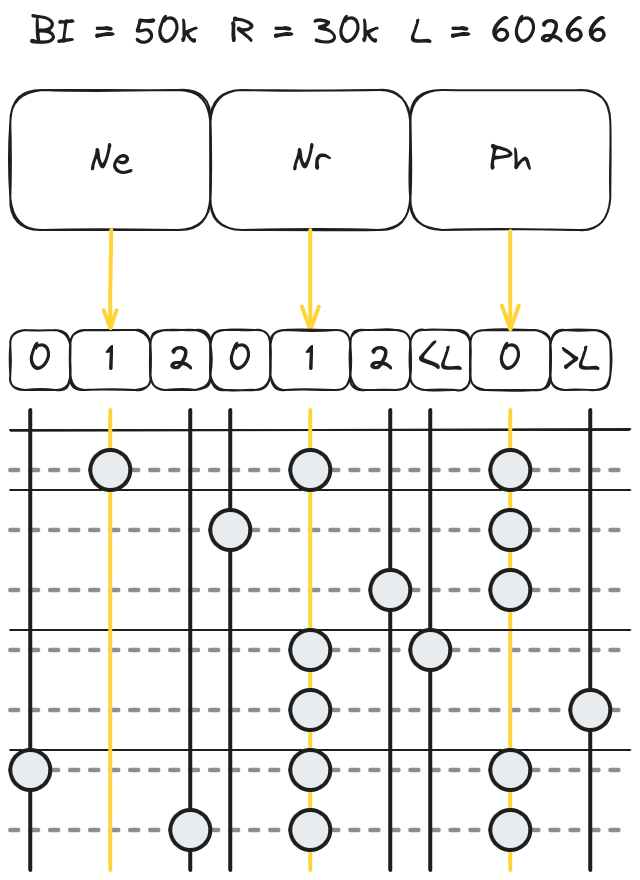
\includegraphics[width=0.5\textwidth]{arbol.png}
	\captionof{figure}{Árbol de decisiones \textit{base choice} con tres variables}
\end{minipage}

La mayoría de situaciones que resultan de la combinación de estas variables ya están
cubiertas por las pruebas de valores límite y clases de equivalencia realizadas anteriormente.
Este estudio demuestra, sin embargo, que se puede llegar a diseñar un sistema más complejo si
se desea alcanzar una mayor cobertura a costa de un gran número de situaciones ya cubiertas.

\input{sections/4_diseño.tex}
\chapter{Preguntas de los enunciados}
\section{Primera entrega}
\subsection{Posibles consecuencias ante un fallo}
\textit{Si este software se tuviera que desplegar en un servicio web accesible a los ciudadanos,
¿qué consecuencias tendría que dicho servicio fallara y no estuviera disponible?}

El fallo de un software de estas características, ya sea por un error en el cálculo de los impuestos, caída
del servicio o cualquier otro problema que afecte al funcionamiento del sistema, puede tener consecuencias
catastróficas para los ciudadanos, ya que el cálculo de los impuestos es un proceso que afecta directamente
a la economía tanto del individuo como del estado.

En caso de fallo, la ciudadanía podría verse afectada por sanciones económicas por parte de la administración
sin justificación ninguna o incluso por la pérdida de dinero en concepto de impuestos que no se deberían haber
pagado. Por otro lado, el estado podría verse afectado por la pérdida de ingresos en concepto de impuestos que
no se han cobrado, lo que podría afectar a la economía del país.

\subsection{Noticias relevantes}
El fallo de software relacionado con administraciones públicas no es ficción, y de hecho es
más que frecuente. A continuación se citan algunas noticias que dejan en evidencia este hecho:
\begin{itemize}
	\item <<El 61\% de los usuarios han tenido problemas al usar las webs o apps de administraciones públicas>>~\cite{newtral}
	\item <<Fallos en los programas y sistemas caídos: programas desactualizados lastran la actividad en Empleo>>~\cite{abc}
	\item <<Sigue sin funcionar>>~\cite{elpais}
\end{itemize}

\newpage{}
\section{Segunda entrega: Aspectos deontológicos}
\textit{¿Qué aspectos deberíamos tener en cuenta como profesionales, desde un punto de vista ético
y deontológico, al diseñar el modo en que se tratan este tipo de ficheros con datos personales y
económicos de ciudadanos por parte de los usuarios del software?}

Como profesionales, debemos tener en cuenta que los datos personales y económicos de los ciudadanos
son información sensible y privada, por lo que debemos garantizar la confidencialidad y seguridad
de los mismos. Para ello, debemos cumplir con la normativa vigente en materia de protección de datos
personales, como el RGPD, y garantizar que los datos se tratan de forma lícita, leal y transparente.

Además, debemos garantizar que los datos se tratan de forma segura, evitando accesos no autorizados
y protegiendo los datos frente a posibles pérdidas o daños. Implementar medidas de seguridad, como
el cifrado de los datos, el control de accesos o la realización de copias, es la mejor estrategia
para garantizar la seguridad de los datos.


%% Esto incluirá la bibliografía correctamente en nuestro trabajo
\newpage % En una nueva página
\addcontentsline{toc}{chapter}{Bibliografía} % Añade la referencia al índice de contenido

\bibliographystyle{ieeetr} % Define el estilo de la bibliografía
\bibliography{biblio} % Indica el archivo que contiene la colección de citas

\nocite{template}
\nocite{sumup}

\end{document}
